\documentclass[10pt]{article}

\usepackage{fullpage}
\usepackage{amsmath}
\usepackage{amssymb}
\usepackage{graphicx}
\usepackage{subfig}
\usepackage{epstopdf}

\begin{document}
\author{
  Thomas \textsc{Debarre}\\
  \texttt{thomas.debarre@gmail.com}
  \and
  Matthieu \textsc{Kirchmeyer}\\
  \texttt{matthieu.kirchmeyer@mines-paristech.fr}
  \and
  Sylvain \textsc{Truong}\\
  \texttt{struong@ens-paris-saclay.fr}
  \and
  Nicolas \textsc{Zhang}\\
  \texttt{nicolas.zhang@mines-paristech.fr}
}
\title{Probabilistic Graphical Models \\ Class Project: progress report}
\maketitle

\section{Problem statement}
This project will explore three methods to solve the problem of word alignments for a bilingual corpus from the conventional mixtures models (IBM1, IBM2) to a first-order HMM model developped in S. Vogel, H. Ney, and C. Tillmann "HMM-based word alignment in statistical translation". The goal is to translate a text given in a language (French in all that follows) to another language (English) taking into account one-to-many alignments; the quality of the translation relies on the quality of the word alignments.

We created a small bilingual French-English dataset $\mathcal{D} = \{ (\mathbf{f}^{(1)},\mathbf{e}^{(1)}), \dots , (\mathbf{f}^{(N)},\mathbf{e}^{(N)})\}$ which consists of $N = 22$ French sentences composed of 4 to 10 words with their translated English equivalents. We evaluated the performance of IBM Model 1 on this dataset. 

\section{First implementation results: IBM Model 1}

\subsection{Description of the algorithm}
The goal of the different algorithms described in this paper is to use a probabilistic model to derive, for any pair of French and English words $(f,e)$ which are part of the training dataset, the conditional probability $p(f \vert e)$. We represent a French sentence $\mathbf{f}$ of length $I$ by a string of words $\langle f_1, \ldots, f_I \rangle$. Similarly, we represent an English sentence $\mathbf{e}$ of length $J$ by a string of words $\langle e_1, \ldots, e_J \rangle$. We assume that each French word is aligned to a single English word, and we call $a_i \in [1, J]$ the alignment variable ($f_i$ is aligned with $e_{a_i}$). In these models, the joint probability of the French sentence and its alignment conditioned on the corresponding English sentence is:
\begin{equation}
p(\mathbf{f}, \mathbf{a} \vert \mathbf{e}) = p(I \vert J) \prod_{i=1}^I p(a_i \vert J) \cdot p(f_i \vert e_{a_i})
\end{equation}
where $\mathbf{a} = \langle a_1, \ldots, a_I \rangle$ is the vector of all alignment variables in the sentence. The latter are \textit{latent variables}, since they are unobserved. The sentence lengths $I$ and $J$ being observed, the conditional probability $p(I \vert J)$ is very easy to estimate. However, estimating $p(f \vert e)$ is a much harder task, since the alignment $\mathbf{a}$ is unobserved.

The difference between the models presented here lies in the assumptions concerning the alignment probabilities. In the case of IBM1, we assume that $p(a_i = j \vert J) = \frac{1}{J}$ for any $i \in [1,I]$ and $j \in [1,J]$, which entails that for 2 corresponding sentences $(\mathbf{f}, \mathbf{e})$, each French word in $\mathbf{f}$ has an equal probability of being aligned with any English word in $\mathbf{e}$. Following this assumption, if the alignment variables were observed, it can be shown that the maximum likelihood estimator of the parameters would be  $\hat{p}(f \vert e) \propto count \langle f, e \rangle$, where $count \langle f, e \rangle$ is the number of times the words $f$ and $e$ are aligned in $\mathcal{D}$. However, since the alignments are latent variables, we do not have access to the $count$ function; hence, we replace it with its expected value $\mathbb{E}(count \langle f, e \rangle)$ in order to use the EM algorithm.

The E-step of the EM algorithm therefore consists here in updating the expected value of the $count$ function $\mathbb{E}(count \langle f,e \rangle)$ for all $(f,e)$ appearing in the training dataset using the estimators of the conditional probabilities $\hat{p}(f \vert e)$ from the M-step of the previous iteration. Next, the M-step updates these $\hat{p}(f \vert e)$ parameters using $\hat{p}(f \vert e) \propto \mathbb{E}(count \langle f,e \rangle)$.

\subsection{First results}
We implemented the IBM1 algorithm on our small dataset of 22 translated sentences. Figure \ref{examples} plots the results (most probable alignments) for a few example sentences.
\begin{figure}[h!]
\centering
\subfloat{\includegraphics[width=.49\textwidth]{1.eps}}
\subfloat{\includegraphics[width=.49\textwidth]{2.eps}} \\
\subfloat{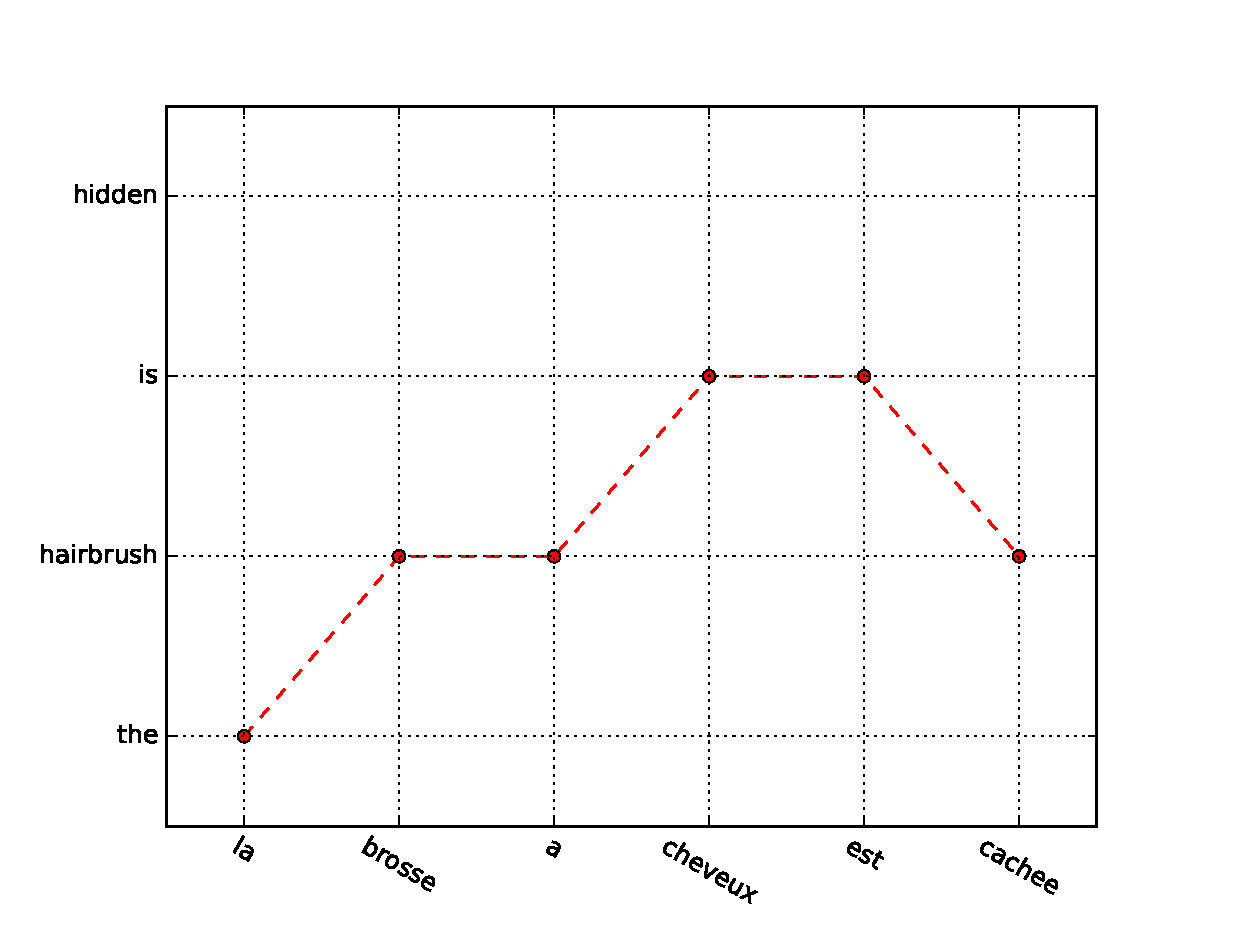
\includegraphics[width=.49\textwidth]{3.eps}}
\subfloat{\includegraphics[width=.49\textwidth]{4.eps}}
\caption{Most probable alignments for 4 example sentences}
\label{examples}
\end{figure}

The algorithm has rather satisfactory results. However, some problems remain, in part due to the small size of our database (some words appear only once), but also to the fact that the position of the word in the sentence is irrelevant (in the 2\textsuperscript{nd} example, the word "the" appears twice, but "le" is mapped to the first one twice). This kind of problem can hopefully be solved with the IBM Model 2 algorithm and the HMM model.

\subsection{Future work}
In the next weeks we will implement 2 other models: IBM Model 2 which extends IBM Model 1 and a HMM model described in the article.

The IBM Model 2 adds a locality information to the lexical information brought by IBM Model 1. This is achieved by adding an absolute reordering model which aligns each output word to the corresponding foreign input position once the lexical translation step (cf. IBM Model 1) is done.

However, one of the main flaws in the IBM Model 1 lies in the locality information as it considers each word to be moving independently, which is often not the case. The HMM model brings an improvement by making the probabilities in the alignment model dependent on the differences in the alignment positions rather than on absolute positions. This allows words to move in clusters and somehow modifies the algorithms behind; for instance it makes dynamic programming necessary in the EM steps.

If time remains we would consider probabilistic context-free grammars and implement algorithms involving fertility (the context, the grammar,...) which have not been mentioned in this report.

\end{document}
